go的安全保护机制分为动态和静态检查两部分。

\begin{enumerate}
\tightlist
\item
  静态如类型检查
\item
  动态如数组越界
\end{enumerate}

另外在go中无法获得goroutine所在的实际线程id,因为go会在不同的时候调度不同的线程给goroutine去运行。也不能获取指针对应的内存地址。因为在不同的时候资源回收之后,动态内存管理可能挪动数据位置,实际指针地址会发生变动。

\hypertarget{unsafe-package}{%
\section{unsafe package}\label{unsafe-package}}

\hypertarget{ux4e3aux4ec0ux4e48ux8981ux4f7fux7528ux8fd9ux4e9bux4f4eux7ea7ux7684ux7f16ux7a0bux63a5ux53e3}{%
\subsection{为什么要使用这些低级的编程接口}\label{ux4e3aux4ec0ux4e48ux8981ux4f7fux7528ux8fd9ux4e9bux4f4eux7ea7ux7684ux7f16ux7a0bux63a5ux53e3}}

\begin{enumerate}
\tightlist
\item
  效率
\item
  和其它语言库交互
\item
  实现不能由纯go语言实现的函数
\end{enumerate}

\hypertarget{unsafe-package-1}{%
\subsection{unsafe package}\label{unsafe-package-1}}

\begin{enumerate}
\tightlist
\item
  是由编译器实现的。
\item
  暴露了go的内存结构。
\end{enumerate}

\hypertarget{unsafe.sizeof-alignof-and-offsetof}{%
\section{unsafe.Sizeof, Alignof, and
Offsetof}\label{unsafe.sizeof-alignof-and-offsetof}}

\hypertarget{sizeof}{%
\subsection{Sizeof}\label{sizeof}}

\begin{enumerate}
\tightlist
\item
  Sizeof只报告数据结构里面的固定部分大小。比如字符串的指针和长度。而字符串具体占用了多大空间则不会报告。
\item
  Sizeof报告的大小,最小是里面固定字段的大小总和。会多余是因为字节对齐。
\end{enumerate}

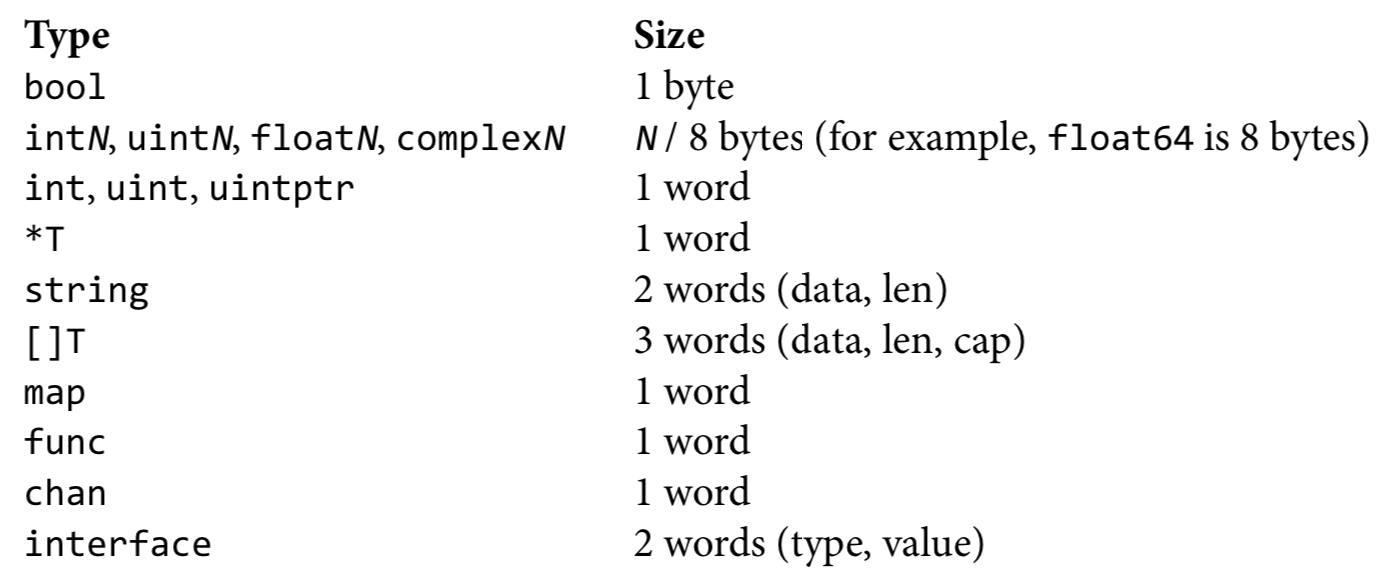
\includegraphics{./ch13/unsafe.Sizeof,_Alignof,_and_Offsetof/screenshot_2019-10-14_08-49-08.png}

\begin{enumerate}
\item
  编译器不一定按照你定义字节的顺序来分配内存或对齐。目前的编译器还不会帮你调整更好的顺序。

  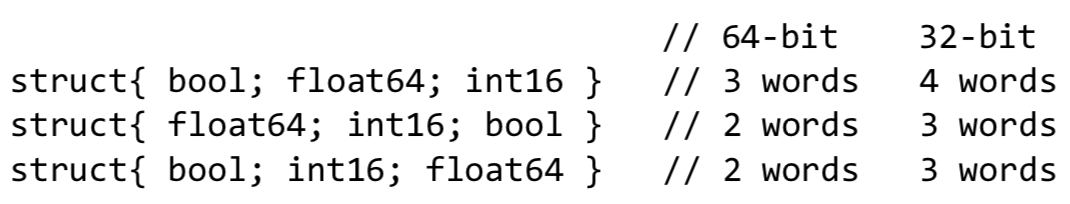
\includegraphics{./ch13/unsafe.Sizeof,_Alignof,_and_Offsetof/screenshot_2019-10-14_08-51-47.png}
\end{enumerate}

\hypertarget{alignof}{%
\subsection{Alignof}\label{alignof}}

参数需要的对齐字节数

\hypertarget{offsetof}{%
\subsection{Offsetof}\label{offsetof}}

参数的偏移地址

\hypertarget{ux603bux7ed3}{%
\subsection{总结}\label{ux603bux7ed3}}

我们来看一个具体的例子。

\begin{Shaded}
\begin{Highlighting}[]
\KeywordTok{var}\NormalTok{ x }\KeywordTok{struct}\NormalTok{ \{}
\NormalTok{  a }\DataTypeTok{bool}
\NormalTok{  b }\DataTypeTok{int16}
\NormalTok{  c []}\DataTypeTok{int}
\NormalTok{\}}
\end{Highlighting}
\end{Shaded}

它的内存结构图

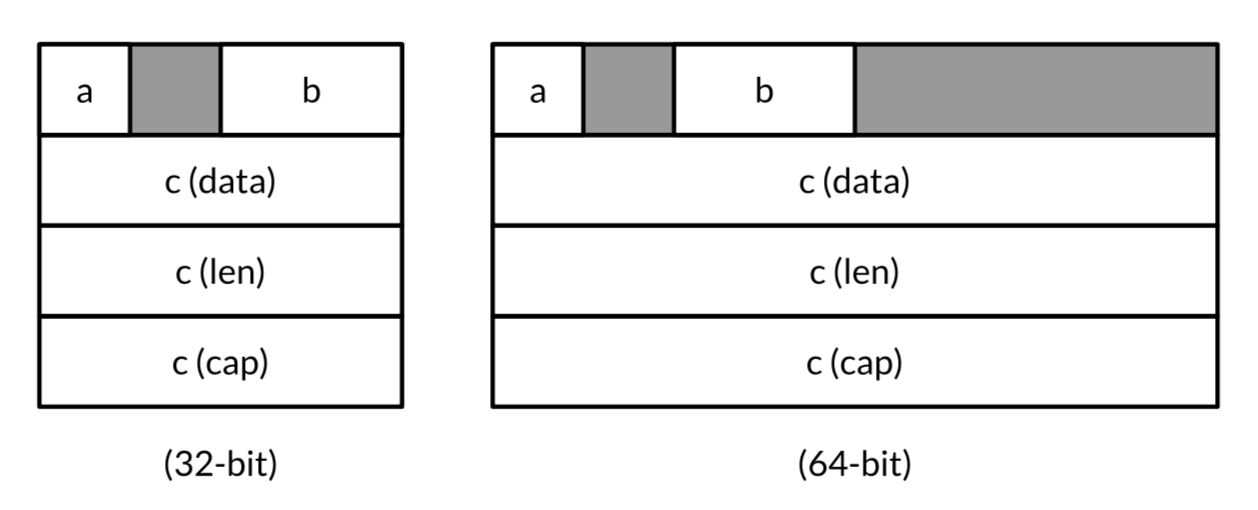
\includegraphics{./ch13/unsafe.Sizeof,_Alignof,_and_Offsetof/screenshot_2019-10-14_09-06-01.png}

调用三个函数的结果

\begin{Shaded}
\begin{Highlighting}[]
\CommentTok{//Typical 32-bit platform:}
\NormalTok{Sizeof(x)   = }\DecValTok{16}\NormalTok{  Alignof(x)   = }\DecValTok{4}
\NormalTok{Sizeof(x.a) = }\DecValTok{1}\NormalTok{   Alignof(x.a) = }\DecValTok{1}\NormalTok{  Offsetof(x.a) = }\DecValTok{0}
\NormalTok{Sizeof(x.b) = }\DecValTok{2}\NormalTok{   Alignof(x.b) = }\DecValTok{2}\NormalTok{  Offsetof(x.b) = }\DecValTok{2}
\NormalTok{Sizeof(x.c) = }\DecValTok{12}\NormalTok{  Alignof(x.c) = }\DecValTok{4}\NormalTok{  Offsetof(x.c) = }\DecValTok{4}
\CommentTok{//Typical 64-bit platform:}
\NormalTok{Sizeof(x)   = }\DecValTok{32}\NormalTok{  Alignof(x)   = }\DecValTok{8}
\NormalTok{Sizeof(x.a) = }\DecValTok{1}\NormalTok{   Alignof(x.a) = }\DecValTok{1}\NormalTok{  Offsetof(x.a) = }\DecValTok{0}
\NormalTok{Sizeof(x.b) = }\DecValTok{2}\NormalTok{   Alignof(x.b) = }\DecValTok{2}\NormalTok{  Offsetof(x.b) = }\DecValTok{2}
\NormalTok{Sizeof(x.c) = }\DecValTok{24}\NormalTok{  Alignof(x.c) = }\DecValTok{8}\NormalTok{  Offsetof(x.c) = }\DecValTok{8}
\end{Highlighting}
\end{Shaded}

\hypertarget{pointer}{%
\section{Pointer}\label{pointer}}

\begin{enumerate}
\tightlist
\item
  常规指针如 *
  T,可以转换为unsafe.Pointer,但是反之则不一定合法。因为你可能讲一个uint16转给一个uint64.这是不合法的。
\end{enumerate}

\begin{Shaded}
\begin{Highlighting}[]
\CommentTok{//通过把浮点64位转为uint64.来看浮点的内存结构}
\KeywordTok{package}\NormalTok{ math}
\KeywordTok{func}\NormalTok{ Float64bits(f }\DataTypeTok{float64}\NormalTok{) }\DataTypeTok{uint64}\NormalTok{ \{ }\KeywordTok{return}\NormalTok{ *(*}\DataTypeTok{uint64}\NormalTok{)(unsafe.Pointer(&f)) \}}
\NormalTok{fmt.Printf(}\StringTok{"%#016x}\CharTok{\textbackslash{}n}\StringTok{"}\NormalTok{, Float64bits(}\DecValTok{1}\FloatTok{.0}\NormalTok{)) }\CommentTok{// "0x3ff0000000000000"}
\end{Highlighting}
\end{Shaded}

\begin{enumerate}
\item
  unsafe.Pointer 也可以转换为 uintptr.

  \begin{itemize}
  \tightlist
  \item
    这个uintptr只是一个数字,指向一个内存地址,这是危险的。因为go的资源回收,可能会移动变量那么
    uintptr指向的位置可能变成一个非法位置。unsafe.Pointer
    却不是这样的,go的内存管理会位置 unsafe.Pointer始终指向正确的位置。
  \item
    有的uintptr值,对应的是不合法的内存值。
  \end{itemize}

  正确代码

\begin{Shaded}
\begin{Highlighting}[]
\NormalTok{gopl.io/ch13/unsafeptr}
\KeywordTok{var}\NormalTok{ x }\KeywordTok{struct}\NormalTok{ \{}
\NormalTok{  a }\DataTypeTok{bool}
\NormalTok{  b }\DataTypeTok{int16}
\NormalTok{  c []}\DataTypeTok{int}\NormalTok{ \}}
\CommentTok{// equivalent to pb := &x.b}
\NormalTok{pb := (*}\DataTypeTok{int16}\NormalTok{)(unsafe.Pointer(}
  \DataTypeTok{uintptr}\NormalTok{(unsafe.Pointer(&x)) + unsafe.Offsetof(x.b)))}
\NormalTok{*pb = }\DecValTok{42}
\NormalTok{fmt.Println(x.b) }\CommentTok{// "42"}
\end{Highlighting}
\end{Shaded}

  错误代码

\begin{Shaded}
\begin{Highlighting}[]
\CommentTok{// }\AlertTok{NOTE}\CommentTok{: subtly incorrect!}
\NormalTok{tmp := }\DataTypeTok{uintptr}\NormalTok{(unsafe.Pointer(&x)) + unsafe.Offsetof(x.b)}
\NormalTok{pb := (*}\DataTypeTok{int16}\NormalTok{)(unsafe.Pointer(tmp))}
\NormalTok{*pb = }\DecValTok{42}
\end{Highlighting}
\end{Shaded}

\begin{Shaded}
\begin{Highlighting}[]
\CommentTok{//错误}
\NormalTok{pT := }\DataTypeTok{uintptr}\NormalTok{(unsafe.Pointer(}\BuiltInTok{new}\NormalTok{(T))) }\CommentTok{// }\AlertTok{NOTE}\CommentTok{: w}
\CommentTok{// 资源回收了但是pT还指向一个错误的位置}
\end{Highlighting}
\end{Shaded}
\item
  call 外部库的时候。应该立即将uintptr转换为unsafe.Pointer

\begin{Shaded}
\begin{Highlighting}[]
\KeywordTok{package}\NormalTok{ reflect}
\KeywordTok{func}\NormalTok{ (Value) Pointer() }\DataTypeTok{uintptr}
\KeywordTok{func}\NormalTok{ (Value) UnsafeAddr() }\DataTypeTok{uintptr}
\KeywordTok{func}\NormalTok{ (Value) InterfaceData() [}\DecValTok{2}\NormalTok{]}\DataTypeTok{uintptr} \CommentTok{// (index 1)}
\end{Highlighting}
\end{Shaded}
\item
  goroutine的stack会增长,所以会发生移动。所以内存地址是会变动的。
\end{enumerate}

\hypertarget{exampledeep-equivalence}{%
\section{\texorpdfstring{\url{Example:Deep}
Equivalence}{Example:Deep Equivalence}}\label{exampledeep-equivalence}}

在reflect模块中,有一个deep
equivalence.他可以深度比较两个对象的是否相同。对于nil和空的字典比较是不等。比如

\begin{Shaded}
\begin{Highlighting}[]
\KeywordTok{var}\NormalTok{ a, b []}\DataTypeTok{string}\NormalTok{ = }\OtherTok{nil}\NormalTok{, []}\DataTypeTok{string}\NormalTok{\{\}}
\NormalTok{fmt.Println(reflect.DeepEqual(a, b)) }\CommentTok{// "false"}
\KeywordTok{var}\NormalTok{ c, d }\KeywordTok{map}\NormalTok{[}\DataTypeTok{string}\NormalTok{]}\DataTypeTok{int}\NormalTok{ = }\OtherTok{nil}\NormalTok{, }\BuiltInTok{make}\NormalTok{(}\KeywordTok{map}\NormalTok{[}\DataTypeTok{string}\NormalTok{]}\DataTypeTok{int}\NormalTok{)}
\NormalTok{fmt.Println(reflect.DeepEqual(c, d)) }\CommentTok{// "false"}
\end{Highlighting}
\end{Shaded}

我们来自己实现一个deep equal 但稍微不同的是上面的比较我们得出相等

\begin{Shaded}
\begin{Highlighting}[]
\CommentTok{// Package equal provides a deep equivalence relation for arbitrary values.}
\KeywordTok{package}\NormalTok{ equal}

\KeywordTok{import}\NormalTok{ (}
  \StringTok{"reflect"}
  \StringTok{"unsafe"}
\NormalTok{)}

\CommentTok{//!+}
\KeywordTok{func}\NormalTok{ equal(x, y reflect.Value, seen }\KeywordTok{map}\NormalTok{[comparison]}\DataTypeTok{bool}\NormalTok{) }\DataTypeTok{bool}\NormalTok{ \{}
  \KeywordTok{if}\NormalTok{ !x.IsValid() || !y.IsValid() \{}
    \KeywordTok{return}\NormalTok{ x.IsValid() == y.IsValid()}
\NormalTok{  \}}
  \KeywordTok{if}\NormalTok{ x.Type() != y.Type() \{}
    \KeywordTok{return} \OtherTok{false}
\NormalTok{  \}}

  \CommentTok{// ...cycle check omitted (shown later)...}

  \CommentTok{//!-}
  \CommentTok{//!+cyclecheck}
  \CommentTok{// cycle check}
  \KeywordTok{if}\NormalTok{ x.CanAddr() && y.CanAddr() \{}
\NormalTok{    xptr := unsafe.Pointer(x.UnsafeAddr())}
\NormalTok{    yptr := unsafe.Pointer(y.UnsafeAddr())}
    \KeywordTok{if}\NormalTok{ xptr == yptr \{}
      \KeywordTok{return} \OtherTok{true} \CommentTok{// identical references}
\NormalTok{    \}}
\NormalTok{    c := comparison\{xptr, yptr, x.Type()\}}
    \KeywordTok{if}\NormalTok{ seen[c] \{}
      \KeywordTok{return} \OtherTok{true} \CommentTok{// already seen}
\NormalTok{    \}}
\NormalTok{    seen[c] = }\OtherTok{true}
\NormalTok{  \}}
  \CommentTok{//!-cyclecheck}
  \CommentTok{//!+}
  \KeywordTok{switch}\NormalTok{ x.Kind() \{}
  \KeywordTok{case}\NormalTok{ reflect.Bool:}
    \KeywordTok{return}\NormalTok{ x.Bool() == y.Bool()}

  \KeywordTok{case}\NormalTok{ reflect.String:}
    \KeywordTok{return}\NormalTok{ x.String() == y.String()}

  \CommentTok{// ...numeric cases omitted for brevity...}

  \CommentTok{//!-}
  \KeywordTok{case}\NormalTok{ reflect.Int, reflect.Int8, reflect.Int16, reflect.Int32,}
\NormalTok{    reflect.Int64:}
    \KeywordTok{return}\NormalTok{ x.Int() == y.Int()}

  \KeywordTok{case}\NormalTok{ reflect.Uint, reflect.Uint8, reflect.Uint16, reflect.Uint32,}
\NormalTok{    reflect.Uint64, reflect.Uintptr:}
    \KeywordTok{return}\NormalTok{ x.Uint() == y.Uint()}

  \KeywordTok{case}\NormalTok{ reflect.Float32, reflect.Float64:}
    \KeywordTok{return}\NormalTok{ x.Float() == y.Float()}

  \KeywordTok{case}\NormalTok{ reflect.Complex64, reflect.Complex128:}
    \KeywordTok{return}\NormalTok{ x.Complex() == y.Complex()}
  \CommentTok{//!+}
  \KeywordTok{case}\NormalTok{ reflect.Chan, reflect.UnsafePointer, reflect.Func:}
    \KeywordTok{return}\NormalTok{ x.Pointer() == y.Pointer()}

  \KeywordTok{case}\NormalTok{ reflect.Ptr, reflect.Interface:}
    \KeywordTok{return}\NormalTok{ equal(x.Elem(), y.Elem(), seen)}

  \KeywordTok{case}\NormalTok{ reflect.Array, reflect.Slice:}
    \KeywordTok{if}\NormalTok{ x.Len() != y.Len() \{}
      \KeywordTok{return} \OtherTok{false}
\NormalTok{    \}}
    \KeywordTok{for}\NormalTok{ i := }\DecValTok{0}\NormalTok{; i < x.Len(); i++ \{}
      \KeywordTok{if}\NormalTok{ !equal(x.Index(i), y.Index(i), seen) \{}
        \KeywordTok{return} \OtherTok{false}
\NormalTok{      \}}
\NormalTok{    \}}
    \KeywordTok{return} \OtherTok{true}

  \CommentTok{// ...struct and map cases omitted for brevity...}
  \CommentTok{//!-}
  \KeywordTok{case}\NormalTok{ reflect.Struct:}
    \KeywordTok{for}\NormalTok{ i, n := }\DecValTok{0}\NormalTok{, x.NumField(); i < n; i++ \{}
      \KeywordTok{if}\NormalTok{ !equal(x.Field(i), y.Field(i), seen) \{}
        \KeywordTok{return} \OtherTok{false}
\NormalTok{      \}}
\NormalTok{    \}}
    \KeywordTok{return} \OtherTok{true}

  \KeywordTok{case}\NormalTok{ reflect.Map:}
    \KeywordTok{if}\NormalTok{ x.Len() != y.Len() \{}
      \KeywordTok{return} \OtherTok{false}
\NormalTok{    \}}
    \KeywordTok{for}\NormalTok{ _, k := }\KeywordTok{range}\NormalTok{ x.MapKeys() \{}
      \KeywordTok{if}\NormalTok{ !equal(x.MapIndex(k), y.MapIndex(k), seen) \{}
        \KeywordTok{return} \OtherTok{false}
\NormalTok{      \}}
\NormalTok{    \}}
    \KeywordTok{return} \OtherTok{true}
    \CommentTok{//!+}
\NormalTok{  \}}
  \BuiltInTok{panic}\NormalTok{(}\StringTok{"unreachable"}\NormalTok{)}
\NormalTok{\}}

\CommentTok{//!-}

\CommentTok{//!+comparison}
\CommentTok{// Equal reports whether x and y are deeply equal.}
\CommentTok{//!-comparison}
\CommentTok{//}
\CommentTok{// Map keys are always compared with ==, not deeply.}
\CommentTok{// (This matters for keys containing pointers or interfaces.)}
\CommentTok{//!+comparison}
\KeywordTok{func}\NormalTok{ Equal(x, y }\KeywordTok{interface}\NormalTok{\{\}) }\DataTypeTok{bool}\NormalTok{ \{}
\NormalTok{  seen := }\BuiltInTok{make}\NormalTok{(}\KeywordTok{map}\NormalTok{[comparison]}\DataTypeTok{bool}\NormalTok{)}
  \KeywordTok{return}\NormalTok{ equal(reflect.ValueOf(x), reflect.ValueOf(y), seen)}
\NormalTok{\}}

\KeywordTok{type}\NormalTok{ comparison }\KeywordTok{struct}\NormalTok{ \{}
\NormalTok{  x, y unsafe.Pointer}
\NormalTok{  t    reflect.Type}
\NormalTok{\}}

\CommentTok{//!-comparison}

\end{Highlighting}
\end{Shaded}

\hypertarget{calling-c-code-with-cgo}{%
\section{Calling C Code with cgo}\label{calling-c-code-with-cgo}}

有两个包可以用来处理调用不同代码的一个是cgo,一个是SWIG(更复杂)

\hypertarget{ux8c03ux7528c}{%
\subsection{调用C}\label{ux8c03ux7528c}}

\begin{enumerate}
\tightlist
\item
  如果简单,可以考虑用go实现
\item
  如果不太复杂,可以考虑用子进程的方法调用
\item
  复杂,和灵活的调用使用cgo
\end{enumerate}

\hypertarget{import-c}{%
\subsection{import C}\label{import-c}}

\begin{enumerate}
\tightlist
\item
  C不是一个包,而是一个预处理命令。运行在编译之前。
\end{enumerate}

\begin{Shaded}
\begin{Highlighting}[]
\CommentTok{// Package bzip provides a writer that uses bzip2 compression (bzip.org).}
\KeywordTok{package}\NormalTok{ bzip}
\CommentTok{/*}
\CommentTok{     #cgo CFLAGS: -I/usr/include}
\CommentTok{     #cgo LDFLAGS: -L/usr/lib -lbz2}
\CommentTok{     #include <bzlib.h>}
\CommentTok{     int bz2compress(bz_stream *s, int action,}
\CommentTok{                     char *in, unsigned *inlen, char *out, unsigned *outlen);}
\CommentTok{ */}
\KeywordTok{import} \StringTok{"C"}

\KeywordTok{import}\NormalTok{ ( }\StringTok{"io"}
  \StringTok{"unsafe"}\NormalTok{ )}
\KeywordTok{type}\NormalTok{ writer }\KeywordTok{struct}\NormalTok{ \{}
\NormalTok{  w      io.Writer }\CommentTok{// underlying output stream}
\NormalTok{  stream *C.bz_stream}
\NormalTok{  outbuf [}\DecValTok{64}\NormalTok{ * }\DecValTok{1024}\NormalTok{]}\DataTypeTok{byte}
\NormalTok{\}}
\CommentTok{// NewWriter returns a writer for bzip2-compressed streams.}
\KeywordTok{func}\NormalTok{ NewWriter(out io.Writer) io.WriteCloser \{}
  \KeywordTok{const}\NormalTok{ (}
\NormalTok{    blockSize  = }\DecValTok{9}
\NormalTok{    verbosity = }\DecValTok{0}
\NormalTok{    workFactor = }\DecValTok{30}
\NormalTok{  )}
\NormalTok{  w := &writer\{w: out, stream: }\BuiltInTok{new}\NormalTok{(C.bz_stream)\}}
\NormalTok{  C.BZ2_bzCompressInit(w.stream, blockSize, verbosity, workFactor)}
  \KeywordTok{return}\NormalTok{ w}
\NormalTok{\}}

\end{Highlighting}
\end{Shaded}

\hypertarget{ux5de5ux4f5cux539fux7406}{%
\subsubsection{工作原理}\label{ux5de5ux4f5cux539fux7406}}

\begin{enumerate}
\tightlist
\item
  cgo会生成一个临时的包
\item
  cgo会调用C编译器去编译处理
\item
  最后这些可用的部分会放到C中。调用者只要调用这个C就可以了。
\item
  可以是用\#cgo,在注释中引入编译选项。
\end{enumerate}

\hypertarget{ux66f4ux591a}{%
\subsection{更多}\label{ux66f4ux591a}}

\begin{enumerate}
\tightlist
\item
  当然也可以把go的东西编译为静态库或者动态库,供C调用。
\item
  cgo的内容非常多,更多参考\href{https://golang.org/cmd/cgo}{cgo}
\item
  cap是容量的,和len的不同在于。len是长度,是现有data的长度。cap是最多可以容纳的极限。
\end{enumerate}

\hypertarget{another-word-of-caution}{%
\section{Another Word of Caution}\label{another-word-of-caution}}

unsafe模块比reflect模块更不建议使用。使用的时候要更为慎重
